\documentclass[12pt]{article}
\usepackage{graphicx}
\usepackage{epstopdf}
\usepackage{float}
\usepackage[a4paper, margin=2.5cm, twocolumn]{geometry}
\usepackage{pdfpages}
\usepackage{amsmath}
\usepackage{bm}
% \usepackage{minted}
% \usepackage{sourcecodepro}
% \usepackage{hyperref}
% \usepackage{multirow}
% \usepackage{rotating}
\usepackage[section]{algorithm}
\usepackage{algpseudocode}
\usepackage[backend=bibtex,bibstyle=ieee,citestyle=numeric-comp]{biblatex}

\bibliography{refs}

\newcommand{\vect}[1]{\bm{#1}}
\newcommand{\mat}[1]{\mathbf{#1}}

\begin{document}\sloppy
\title{Parallel Adaptation of Orthotree Meshes \\ . \\ Technical Milestone Report}
\date{14th November 2016}
\author{Matt Diesel (md639) \\ St. Catharine's \\ CCN: 5540D \\ . \\ Supervisor: Dr. Jie Li}

% \includepdf[pages={-}]{cover.pdf}

\maketitle

\begin{abstract}
An extension to current Fully Threaded Tree (FTT) implementations is presented, which retains the benefits of the underlying FTT for Adaptive Mesh Refinement (AMR) methods whilst allowing it to be stored and evaluated in parallel. Distribution using space filling curves has been investigated, with the Hilbert curve proving to be a good solution with minimal computation cost. Distribution and rebalancing of the tree using the Hilbert distribution has been developed and proven on a moving mesh, whilst methods for adaptation and refinement in parallel have been proposed. All methods have been written generalised to both 2d and 3d cases, though testing has only taken place on the 2d case. The implementation has not been optimised or benchmarked against current scatter and gather parallel techniques, or been tested using fluid solvers. 
\end{abstract}

\section{Introduction}
Adaptive Mesh Refinement (AMR) is a commonly used method for evaluating fluid problems. Current methods for solving problems in parallel rely on a single processing unit for adaptation and refinement, before scattering and gathering to evaluate the tree. In Khokhlov's analysis of his FTT implementation given in \cite{Khokhlov98} he concludes that between $10-15\%$ of the algorithm time was spent on gather+scatter of the tree. For this project, an alternative method where subsets of the tree are stored on each processor is investigated, with rebalancing when required. This method should provide some benefit over conventional scatter+gather techniques especially in cases where the cost of data transfer between processing units is high. It also removes the memory restriction on the tree having to fit within a single processing units memory, allowing for the number of cells in a simulation to be increased by a factor of the number of processing units. 

Although the solution has been developed from scratch, the interface is highly similar to that of existing Fully Threaded Tree (FTT) implementations, and so integrating existing solvers designed for adaptive methods is trivial. Should it prove successful, integration into current solver packages such as Gerris should be possible.

\section{Orthotree Fundamentals}
\label{orthotree}
An orthotree is an N dimensional tree structure, where each cell is orthotopic \cite{coxeter73} and its children are evenly sized similar orthotopes. For the purpose of this report, the 2d case (a Quadtree) is explained in detail, with reference to 3d Octrees where generalisation to higher dimensions is non-trivial. 

Orthotrees obey the following criterion:
\begin{enumerate}
	\item The computational domain is the orthotope completely containing the problem
	\item The root of the tree is the cell representing the computational domain.
	\item Each cell has a pointer to its children cells, or nil if it has no children in which case it is referred to as a leaf.
	\item A cells depth is the number of parent links that need to be followed to reach the root of the tree.
	\item Each tier of the tree is the set of cells at that depth.
\end{enumerate}

A number of additional constraints are added to make the orthotree more suitable for solving fluid simulation problems:
\begin{enumerate}
	\item Neighbouring cells may be no more than one tier apart, this is known as 2:1 balancing, though that term won't be used in this document to avoid confusion with balancing across processor units.
	\item There is a finite limit on the depth of the tree.
	\item There is a minimum depth of the tree.
\end{enumerate}

Finally a number of conventions are used both in this document and in the reference implementation:
\begin{enumerate}
	\item Child numbering is done using one bit per dimension, starting from the least significant bit (LSB) and a 1 indicating the cell is in the positive orthant. 
	\item Neighbour and cell face ordering is done such that the LSB is the orthant in the same way as child numbering, whilst the remaining bits give the dimension number.
\end{enumerate}

\subsection{FTT Fundamentals}
A Fully Threaded Tree (FTT) is an extension of the Orthotree structure, in which more links are maintained within the tree. This speeds up access to adjacent cells within the tree from $O(\log(N))$ to $O(1)$, since fetching neighbours is used in every cell evaluation in finite difference methods, this optimisation is a crucial one. 

An FTT implementation is given by Khokhlov in \cite{Khokhlov98}. They present an implementation that minimises the memory requirement of pointers to adjacent cells by a factor of $2^N$ by grouping a cells children into an ortho, with a small amount of extra computation required for some operations. 

The following criterion are added for a FTT implementation:
\begin{enumerate}
	\item An ortho (A "quad" in 2d and an "octo" in 3d) is a grouping of $2^N$ sibling cells with dimensions equal to half of the parent.
	\item Each ortho maintains links to the parent and neighbouring orthos.
	\item Orthos on the computational domain boundary have a special neighbour link, representing either a copy or reflect boundary.
\end{enumerate}

\subsection{Threaded FTT}
The first extension to Khokhlov's FTT implementation in \cite{Khokhlov98} added by this project, in order to efficiently maintain subtrees across multiple processor units, is the addition of another thread through the tree, storing the space filling curve. This is implemented as a doubly linked list of orthos in the tree. This new structure is referred to as a Threaded FTT (TFTT). Double linking is required in order to update not only the link from a cell being modified to its successor, but also from its predecessor. 

The list is maintained for the complete tree available on the processor, so for evaluation purposes the tree stores pointers to the first and last orthos the processor is actively evaluating. Whilst not essential, it was found that this made rebalancing of the tree much simpler, as the stages of the thread before and after the current processing unit is already known.

\subsection{Space Filling Curves}
A space filling curve (SFC) is a path through a every cell in a mesh exactly once. The concept of using a SFC for sequential cell ordering on quadtrees has been explored previously \cite{bader2013} and the concepts can be re\"used here with minor modification. Rather than the SFC being used as an iterating method over the tree, it is instead used to calculate pointers to the next and previous cells within the tree. This way the curve is maintained in memory, and modified as appropriate. 

The two operations that modify the curve are refinement and coarsening of the tree. In the refinement case it is assumed that the previous cell to the one being refined will, after refinement, point to the first child in the orthos SFC, and likewise the next cell will point to the last child. Similarly when coarsening, the cell being coarsened will point to the next cell of the last child and previous cell of the first child. This behaviour is crucial as it implies that refinement and coarsening only changes the space curve locally, and that the SFC for a refined ortho can be generated without knowledge of the rest of the tree.

For this report, the notation used will be a function $\vect{C^N}$ returning a list of child indices (see the conventions in Section \ref{orthotree}) given in the SFC order. This is (optionally) a function of some property $D$ stored with the cell. This notation differs slightly from other notations such as the Lindenmayer rewrite system, but benefits from not needing to work on a complete mesh, or on a single tier. 

For example, the simplest SFC to implement would be the Morton curve, which simply returns the child indices in order:

\begin{equation}
	C_{\mathrm{mort}}^2 \gets \left( 0 \to 1 \to 2 \to 3 \right)
\end{equation}

The Morton curve minimises the computation cost of maintaining the thread, but leads to large gaps between sequential cells in the thread, which when distributing along the thread could lead to a processor unit working on cells in two separate locations.

An alternative space filling curve is the Hilbert Curve, proposed by David Hilbert in 1891 as a curve that guaranteed that sequential cells would always be neighbours. This removes any possibility of complete separation of the cells in a processor unit, and can be represented using the notation described above with the addition of an orientation property, using the notation introduced by Bader \cite{bader2013} in Chapter 3.1. 

\begin{align}
	C_{\mathrm{hilb}}^2\left(D\right) &\gets \\
	& \begin{cases}
		\left( 0 \to 2 \to 3 \to 1\right) & \text{if }D=H \\
		\left( 3 \to 1 \to 0 \to 2\right) & \text{if }D=C \\
		\left( 0 \to 1 \to 3 \to 2\right) & \text{if }D=A \\
		\left( 3 \to 2 \to 0 \to 1\right) & \text{if }D=B
		\end{cases} \nonumber
\end{align}

Although there is a gray code pattern to the curve, this does not extend into 3d and a lookup table is more appropriate.

On refinement, the orientation of child cells $D_c(D_p)$ is a function of the parent orientation $D_p$ using the production rules given by Bader \cite{bader2013}, rewritten into this documents child order convention, as opposed to his presentation in Hilbert child order. This makes the pattern in the inheritance less obvious, but is more suited to use during the refinement process.

\begin{align}
	D_c(H) \gets& \left( A \to B \to H \to H \right) \\
	D_c(C) \gets& \left( C \to C \to A \to B \right) \\
	D_c(A) \gets& \left( H \to A \to C \to A \right) \\
	D_c(B) \gets& \left( B \to H \to B \to C \right)
\end{align}


In both cases, the Hilbert curve satisfies the requirement that no knowledge of the rest of the tree is required for refinement and coarsening. The Hilbert curve has been defined by a number of independent sources in N dimensions, such as Butz in \cite{butz71}, and can be adapted to the above notation and method of implementation easily retaining similar properties. 

\subsection{SFC Comparison}

In Figure \ref{sfc-mort}, rank 2 can be seen to have two completely separate blocks of cells. The Hilbert curve in Figure \ref{sfc-hilb}, whilst not completely optimal, has more effectively minimised the boundary layer between processing units. An optimal solution would require changing the curve for each iteration, and knowledge of the tree. 

\begin{figure}[H]
\caption{Morton SFC distribution, max depth of 10}
\label{sfc-mort}
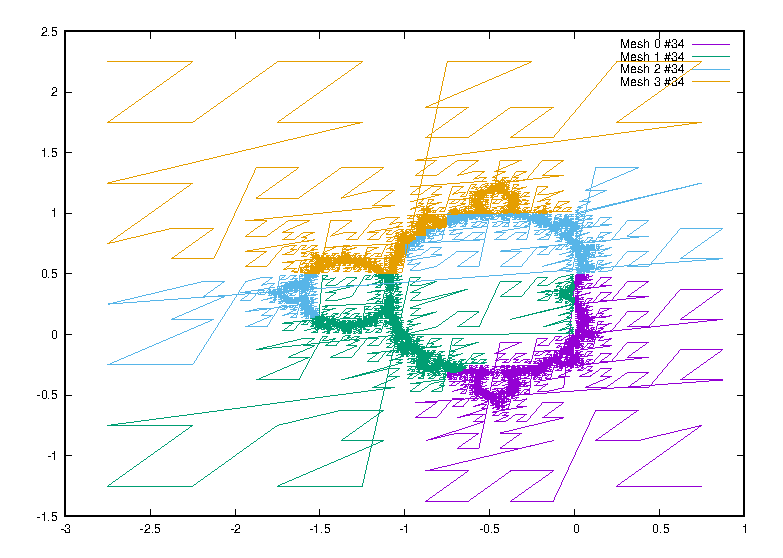
\includegraphics[width=3in]{mort.eps}
\end{figure}

\begin{figure}[H]
\caption{Morton SFC distribution, max depth of 10}
\label{sfc-hilb}
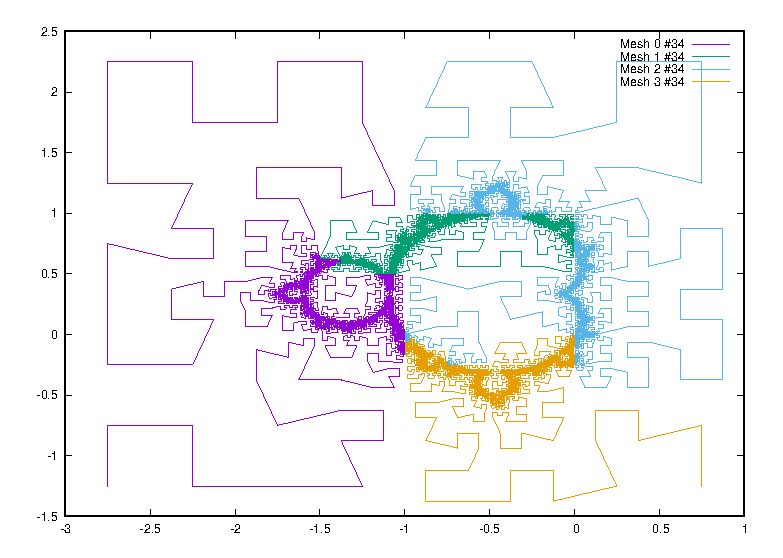
\includegraphics[width=3in]{hilb.eps}
\end{figure}

\subsection{Parallel TFTT}

The final extensions to the tree structure are to allow for the entire process of evaluation and adaptation to be done in parallel. Orthos on the processor boundaries are required by both processors at that boundary. These are referred to as "ghost" orthos on the processor they are not active on. Ghost orthos are present within the tree as normal orthos, but after each time step of the solver the value of cells adjacent to the boundary must be fetched. Processors must therefore maintain a list of the ghost orthos present within their tree, which can change during both rebalancing and refinement. 

To enable inter-process communication, a cell identifier format is implemented that is guaranteed to be unique within the global tree. The method used for the reference implementation encodes both the level and location of the cell, hence uniquely identifying it within the entire tree, and allowing logarithmic lookup time. 

\section{Refinement}

The tree is refined by finding all cells whose refinement indicator $\xi > \xi_{\mathrm{split}}$, and coarsened for cells where $\xi < \xi_{\mathrm{join}}$ as in Khokhlov's AMR method. These indicators are normalised, and highly problem dependent. If the indicator is based on flux between cells, then it is better to store the indicator with the cell and set during the evaluation of the tree, though if it is just a function of a cells value then if does not need to be stored. Refining the whole tree must be done in two steps as given in Algorithm \ref{alg:refine}. First the set of cells to be refined is stored in the list $Q_\mathrm{refine}$, then the cells are refined and the refinement is propagated to enforce the restriction that the difference in tier between adjacent leaves is no more than one. And ghost cells that would be refined are stored, and at the end of each propagation iteration these must be sent to the owning processor unit to be refined.

Although this second step appears to add a lot of complexity and computation cost to the refinement method, it is highly unlikely that more than one iteration is required. This method assumes that the problem is set up such that $\xi$ for is going to change gradually. A rapidly changing $\xi$ could cause a cell to be coarsened and refined in one time step. 

\begin{algorithm}[H]
\caption{Refinement on a Subtree}
\label{alg:refine}

\begin{algorithmic}
\Function{RefineTree}{}
	\State $Q_{\mathrm{ghosts}} \gets \emptyset \text{ , } Q_{\mathrm{refine}} \gets \emptyset$
	\ForAll{tree cells}
		\If {$\xi_{\mathrm{cell}} > \xi_{\mathrm{split}}$}
			\State $Q_{\mathrm{refine}} \gets cell$
		\ElsIf {$\xi_{\mathrm{cell}} < \xi_{\mathrm{join}}$}
			\State \Call{CoarsenCell}{cell}
		\EndIf
	\EndFor
	\Statex
	\Repeat
		\ForAll{$Q_{\mathrm{refine}}$}
			\State \Call{RefinePropagate}{cell}
			\State \Call{RefineCell}{cell}
		\EndFor

		% \ForAll{$Q_{\mathrm{ghosts}}$}
		% 	\State $\text{Send refine message to owning processor}$
		% \EndFor
		\State $Q_\mathrm{ghosts} \to \text{Owning processors}$
		\State $Q_{\mathrm{refine}} \gets \text{refine message from others}$
	\Until {$Q_{\mathrm{refine}} = \emptyset$}
\EndFunction
\end{algorithmic}
\end{algorithm}

\begin{algorithm}
\begin{algorithmic}
\Function{RefinePropagate}{$cell$}
	\ForAll{cell neighbours}
		\If {$Tier_{\mathrm{cell}} > Tier_{\mathrm{neighbour}}$}
			\If {\Call{IsGhost}{$neighbour$}}
				\State $Q_\mathrm{ghosts} \gets neighbour$
			\Else
				\State \Call{RefinePropagate}{$neighbour$}
				\State \Call{RefineCell}{$neighbour$}
			\EndIf
		\EndIf
	\EndFor
\EndFunction
% \Statex
% \Function{refineCell}{$cell$}
% 	\State $Children_{\mathrm{cell}} \gets \text{new ortho}$
% 	\ForAll {children}
% 		\State $\text{Construct child}$
% 		\State $\text{Update FTT}$
% 	\EndFor
% 	\State $\text{Update Curve Thread}$
% \EndFunction
% \Statex
% \Function{coarsenCell}{$cell$}
% 	\State $Children_{\mathrm{cell}} \gets \emptyset$
% \EndFunction
\end{algorithmic}
\end{algorithm}

\section{Rebalancing}

Rebalancing is achieved by calculating on rank zero the average number of cells per processor, and the movement of cells between processors required to achieve a perfect balance. Since the tree is distributed using a space filling curve, the cells can only be passed by the processor to the next of previous. This also implies that a processor can only send or receive cells in a direction, never both. This allows Algorithm \ref{alg:passingcalc} to determine the number of cells each processor passes left and right, and simplifies the interprocess communication.

\begin{algorithm}
\begin{algorithmic}
\caption{Rebalancing Calculations}
\label{alg:passingcalc}

\Function{CalculatePassing}{}
	\State $\vect{c} \gets \text{cell count from processors}$
	\ForAll {processor $p$}
		\State $L_p \gets -R_{p-1}$
		\State $R_p \gets c_p - L_p - \bar{c}$
	\EndFor
\EndFunction

\end{algorithmic}
\end{algorithm}

The rebalancing itself is also simplified by the constraint on processors to only pass to the left or right. The required number of cells are sent or received in each direction and the thread updated. Each cell passed away is guaranteed to become a ghost cell, and any of its neighbours that are themselves ghost cells can be removed from the list of ghosts, as long as they don't border any other active cells. Cells received can must be an existing ghost cell, and any of its neighbours that aren't active on the processor or already marked as ghost cells need to be added to the ghost cell list.

In this way, the rebalancing of the tree, with the exception of the calculations for the pass counts, requires no knowledge of the full tree, only the list of cells being passed to/from the left/right processor. 

\section{Future}
Some work still remains in the implementation of the proposed methods, followed by testing using the existing test cases. Specifically, the method of refinement in parallel is yet to be developed. This should be completed within the first 2 weeks of Lent term. Some testing will need to be done on the 3d specialisation of the structure, as this is yet to be used. 

Following the completion of the structure, test cases similar to those given by Khokhlov in \cite{Khokhlov98} for the 1, 2 and 3 dimensional cases can be used against the proposed extension to the FTT structure, and methods optimised using the runtime on these cases as the fitness function. Following this, the test cases can be compared to an equivalent gather and scatter method of parallel processing. Existing solvers should be able to be re\"used for this, so the whole process should take no more than 4 weeks, including the modification of the tree to use a scatter+gather method, using both passing the full tree structure and scattering leaves according to the SFC. With these tests, some optimisation of parameters can be done, and the structure tweaked as bottlenecks become known. Depending on how efficiently implemented the structure is and what remains to be improved, this could take anywhere between a few days or a few weeks. As a final set of tests, the structure can be compared to an equivalent solver in Gerris or other public CFD programs. 

Some work has been done on the parallel construction of orthotrees by others, such as Sundar et al in \cite{sundar2008}, which would perhaps integrate well into the extended tree proposed here, providing additional benefits over existing methods. Implementation of this is not essential, and will be completed time permitting at the end of the project.

The structure then needs to be documented and made usable as a multi-purpose library. Thought at each stage of the project has gone into this, so adaptation should be simple. This final stage will take place at the same time as final report writing, as there is significant overlap between the documentation and report. 

\section{Conclusion}
The majority of the development work has been done for the proposed structure, with some limited testing to demonstrate the distribution and rebalancing elements. After qualitative testing, the Hilbert curve has shown to be best suited for use in distribution. Extensive testing on fluids simulations remains to be done in Lent term, the results of which will allow an analysis of the new method and will decide its suitability. 


\printbibliography

\end{document}